\section{Исследование}

Для оценки натренированных моделей мы использовали следующие функции ошибки:
\[
    \text{MSE} = \frac{1}{n} \sum_{\substack{x_i, y_i \in \Omega }} \left( NN(x_i, y_i) - u(x_i, y_i) \right)^2,
\]
\[
    \text{MAX} = \max_{x_i,y_i \in \Omega} \left| NN(x_i, y_i) - u(x_i, y_i) \right|.
\]

При подборе гиперпараметра часто используется достаточно небольшое количество эпох, чтобы определить динамику сходимости и погрешности.
Мы не всегда придерживались этого принципа. Например, для демонстрации какой-никакой работоспособности метода для диапазона параметров
в промежутке $[0.3, 20000]$ полученного с помощью функции
\textrm{numpy logspace}, генерирующей последовательность в заданном промежутке, возрастающую экспоненциально, мы тренировали модель в течение
15 000 эпох.

Это дало следующие результаты:

\begin{figure}[ht!]
    \centering
    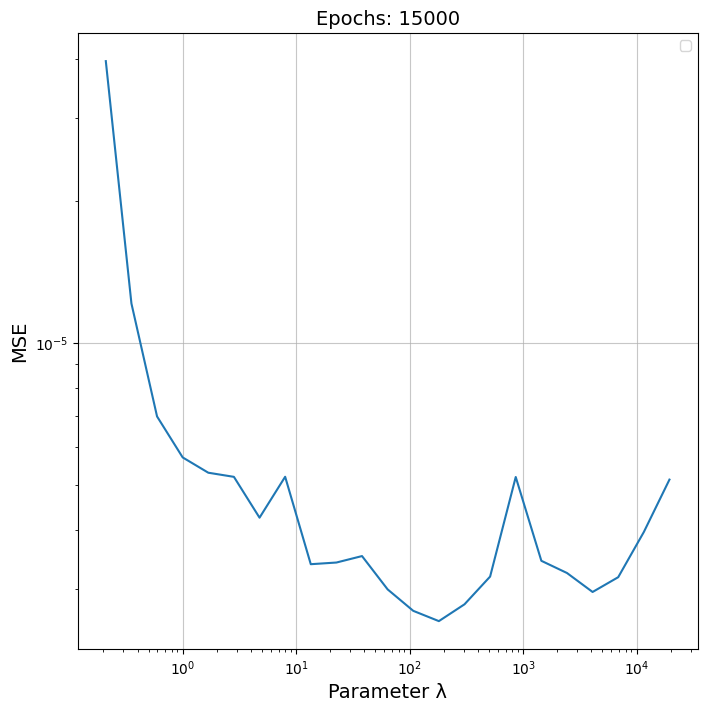
\includegraphics[width=0.9\hsize]{images/1.png}
    \caption{15000 эпох, среднеквадратичная ошибка}
\end{figure}

\begin{figure}[ht!]
    \centering
    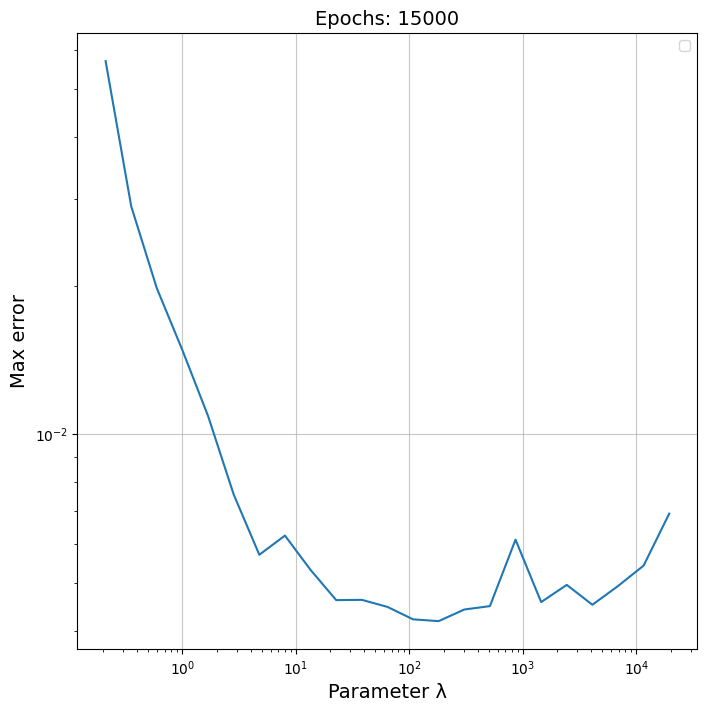
\includegraphics[width=0.9\hsize]{images/2.png}
    \caption{15000 эпох, максимальная ошибка}
\end{figure}

Точные цифры привести, к сожалению, не приведены. Но ошибка, будет видно позже по тепловой карте, не превышает $5e-3$.

\begin{figure}[ht!]
    \centering
    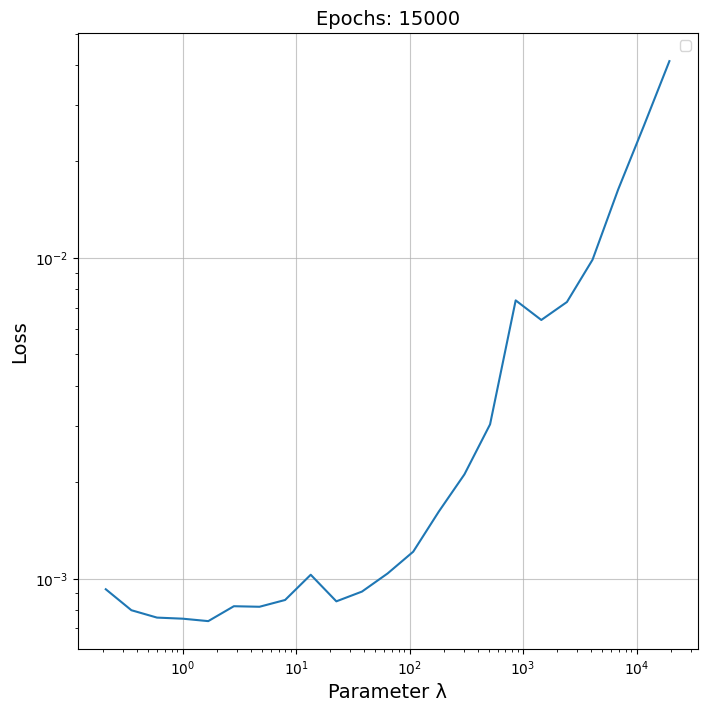
\includegraphics[width=0.9\hsize]{images/6.png}
    \caption{15000 эпох, потери, сходимость}
\end{figure}

Можно сделать, очевидный вывод о том, что меньшее значение функции потерь необязательно приводит к уменьшению ошибки аппроксимации.
Очевидный в силу того, что для больших лямбда функция $L(\omega, \lambda)$ больше из-за роста множителя при второй сумме.

\begin{figure}[ht!]
    \centering
    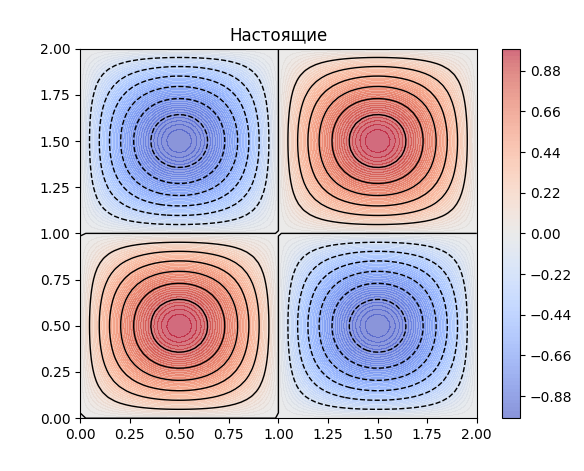
\includegraphics[width=0.5\hsize]{images/3.png}
    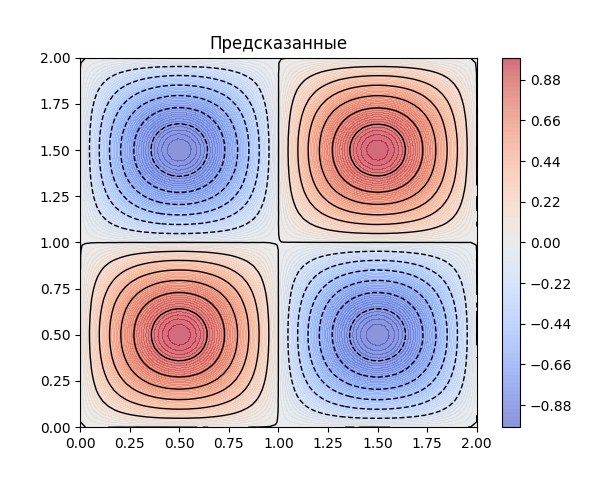
\includegraphics[width=0.5\hsize]{images/4.png}
    \caption{Тепловая карта настоящей функции и значений модели (гиперпараметр неизвестен)}
\end{figure}

\begin{figure}[ht!]
    \centering
    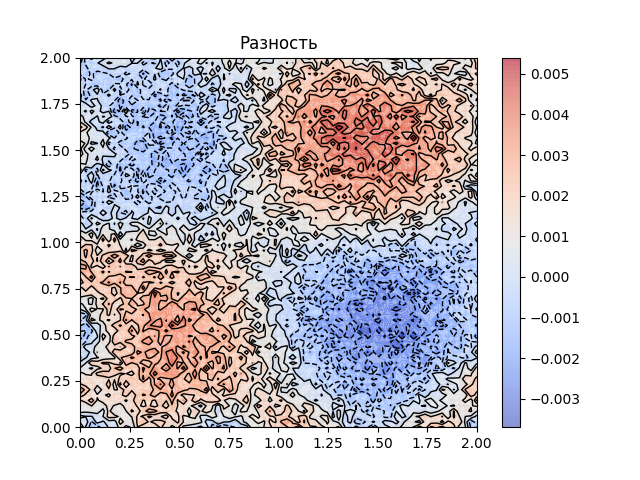
\includegraphics[width=0.9\hsize]{images/19.png}
    \caption{Разница приведенных сверху карт}
\end{figure}

Различие достаточно большое в рамках численных методов, но видно, что нейросеть приближает то, что нужно.

\medskip
\medskip
\medskip
\medskip
